\section{Design}
\label{sec:Design}

\subsection{Database Design} 
Bmob online database was chosen for the relational database management system (RDBMS) for both the Android application and the web interface because it is a free and open source product. The entity relationship (ER) diagram for the whole project is shown in Figure \ref{ERDiagram}.

\begin{figure}[htb]
\centering
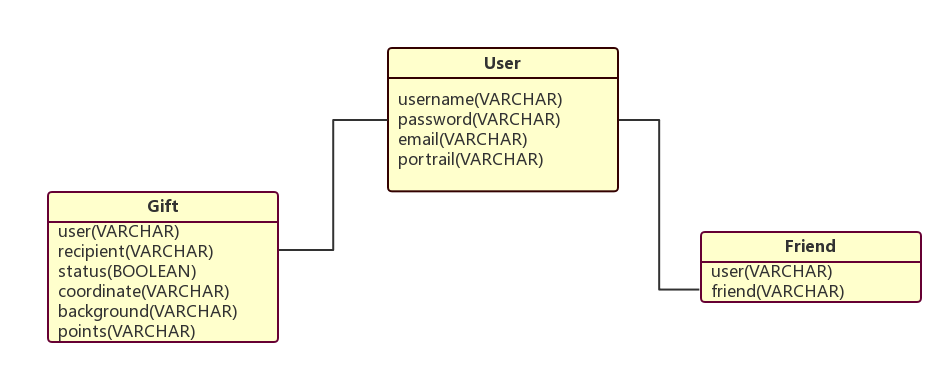
\includegraphics[width=.5\textwidth]{section03/assets/ERDiagram.png}
\caption[Short Caption 2]{\label{ERDiagram}ER Diagram for the project}
\end{figure}

\paragraph{}
All three tables designed for this project are listed in the ER Diagram.
\begin{itemize}
\item The 'User' table will save all the user information. In this table username and email will be unique for each user and this will be verified when users are registered.
\item The 'Friend' table is for saving all friends pairs and both 'user' and 'friend' columns are usernames from 'User' table.
\item The 'Gift' table saves all the gifts information. The 'user' column records the user who sent the gift. The 'recipient' column records the user who will receive the gift. The 'status' column is a boolean type data meaning the gift is found if it is 'true'. The 'coordinate' column is designed to hold the location where the gift was sent. The 'background' column is designed to hold the region picture and the 'points' column is designed to hold the four corners selected by users.
\end{itemize}

\subsection{User Interface Design}
\paragraph{}Following the user interface design principles, especially the accessibility, this user interface is designed to be clear and easy to use. All the parts keeps same color style and try not to use too much colors and fonts so that the user interface is aesthetically pleasing. The main pages are listed below:
\begin{figure}[htb]
\centering
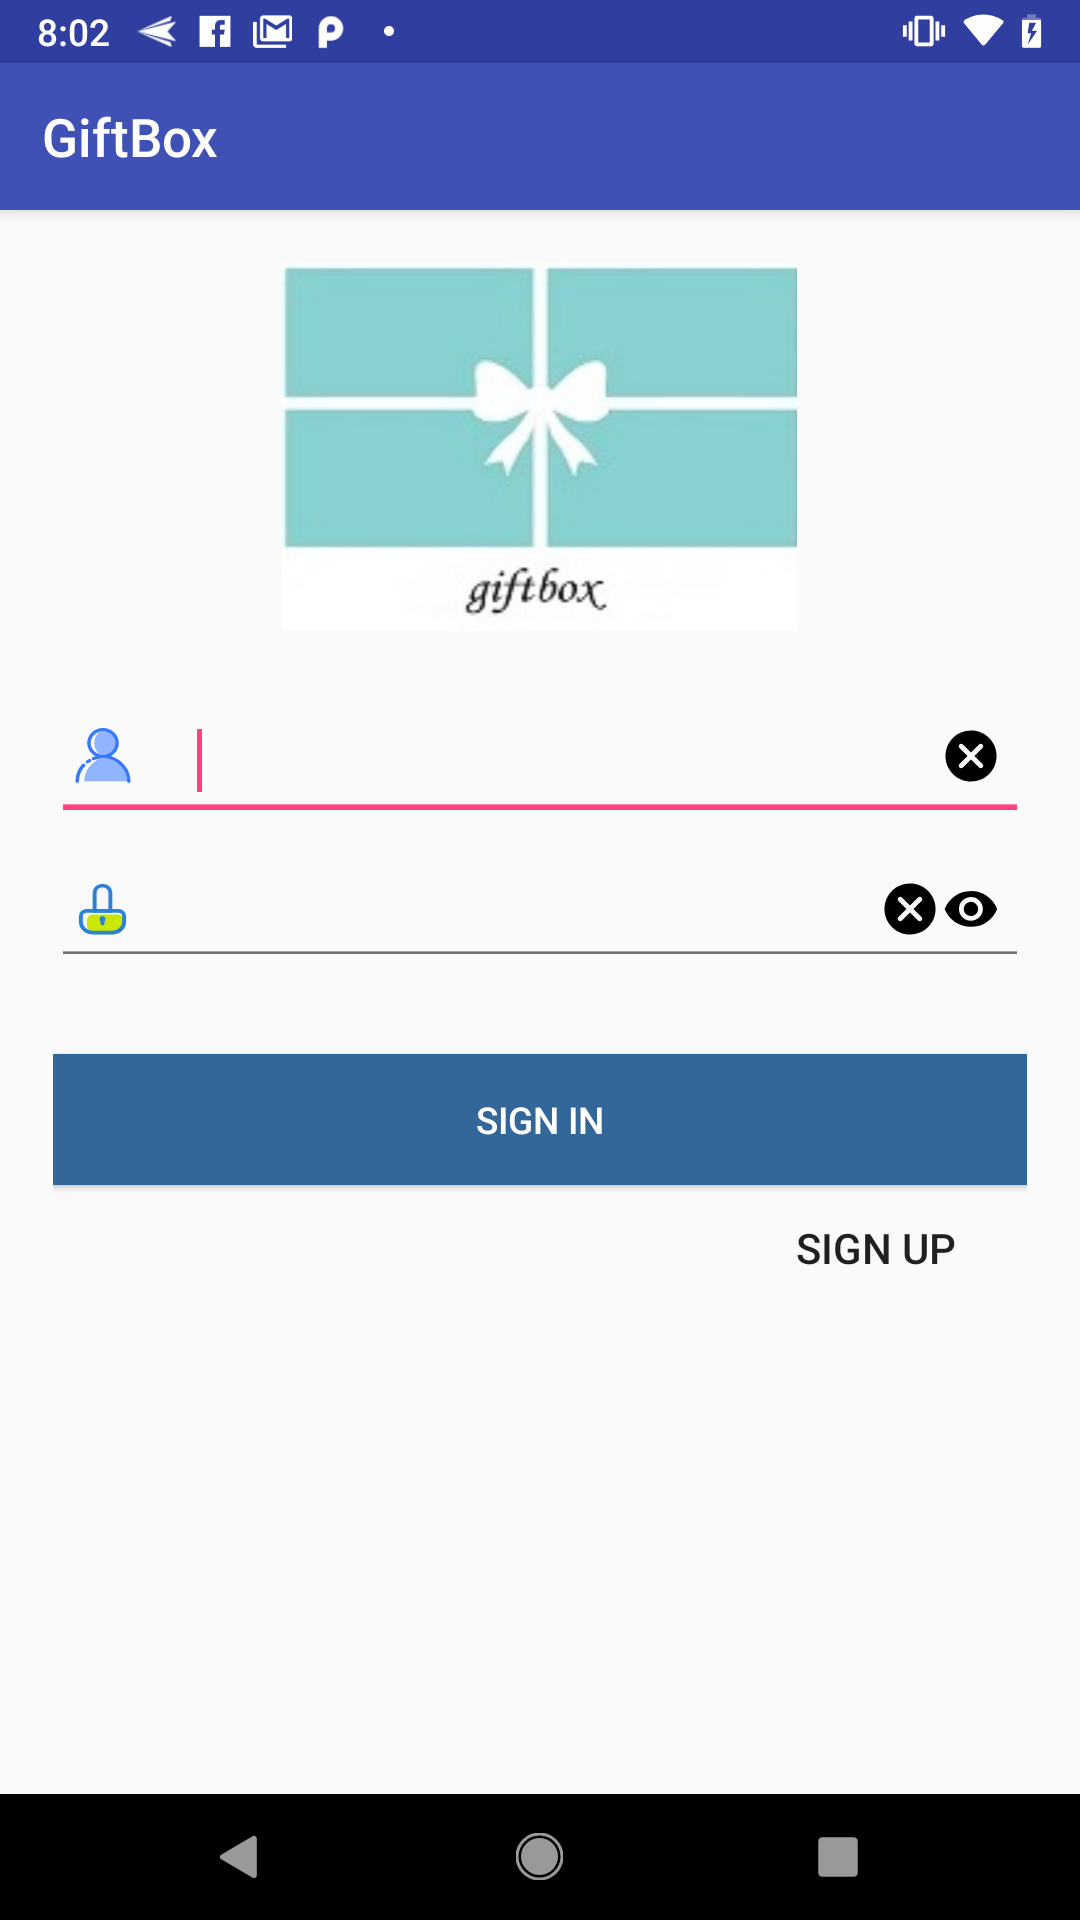
\includegraphics[width=.5\textwidth]{section03/assets/SignIn.png}
\caption[Short Caption 2]{\label{SignInUI}ER Diagram for the project}
\end{figure}
\par The sign in page is shown in Figure \ref{SignInUI}. The logo is designed to show up so that the user will be able to know which application they are using. The user icon and the password icon at the left side of the text field hints to users the meaning of the two fields. The delete icon and the eye icon at the right side of the text field used another color because they have different functions. Users can use the delete button to delete the whole string they typed in and view the password in plain text or encrypted text. The 'Log In' button is designed to be big to prevent users from making mistakes. 

\begin{figure}[htb]
\centering
\begin{minipage}[t]{0.5\textwidth}
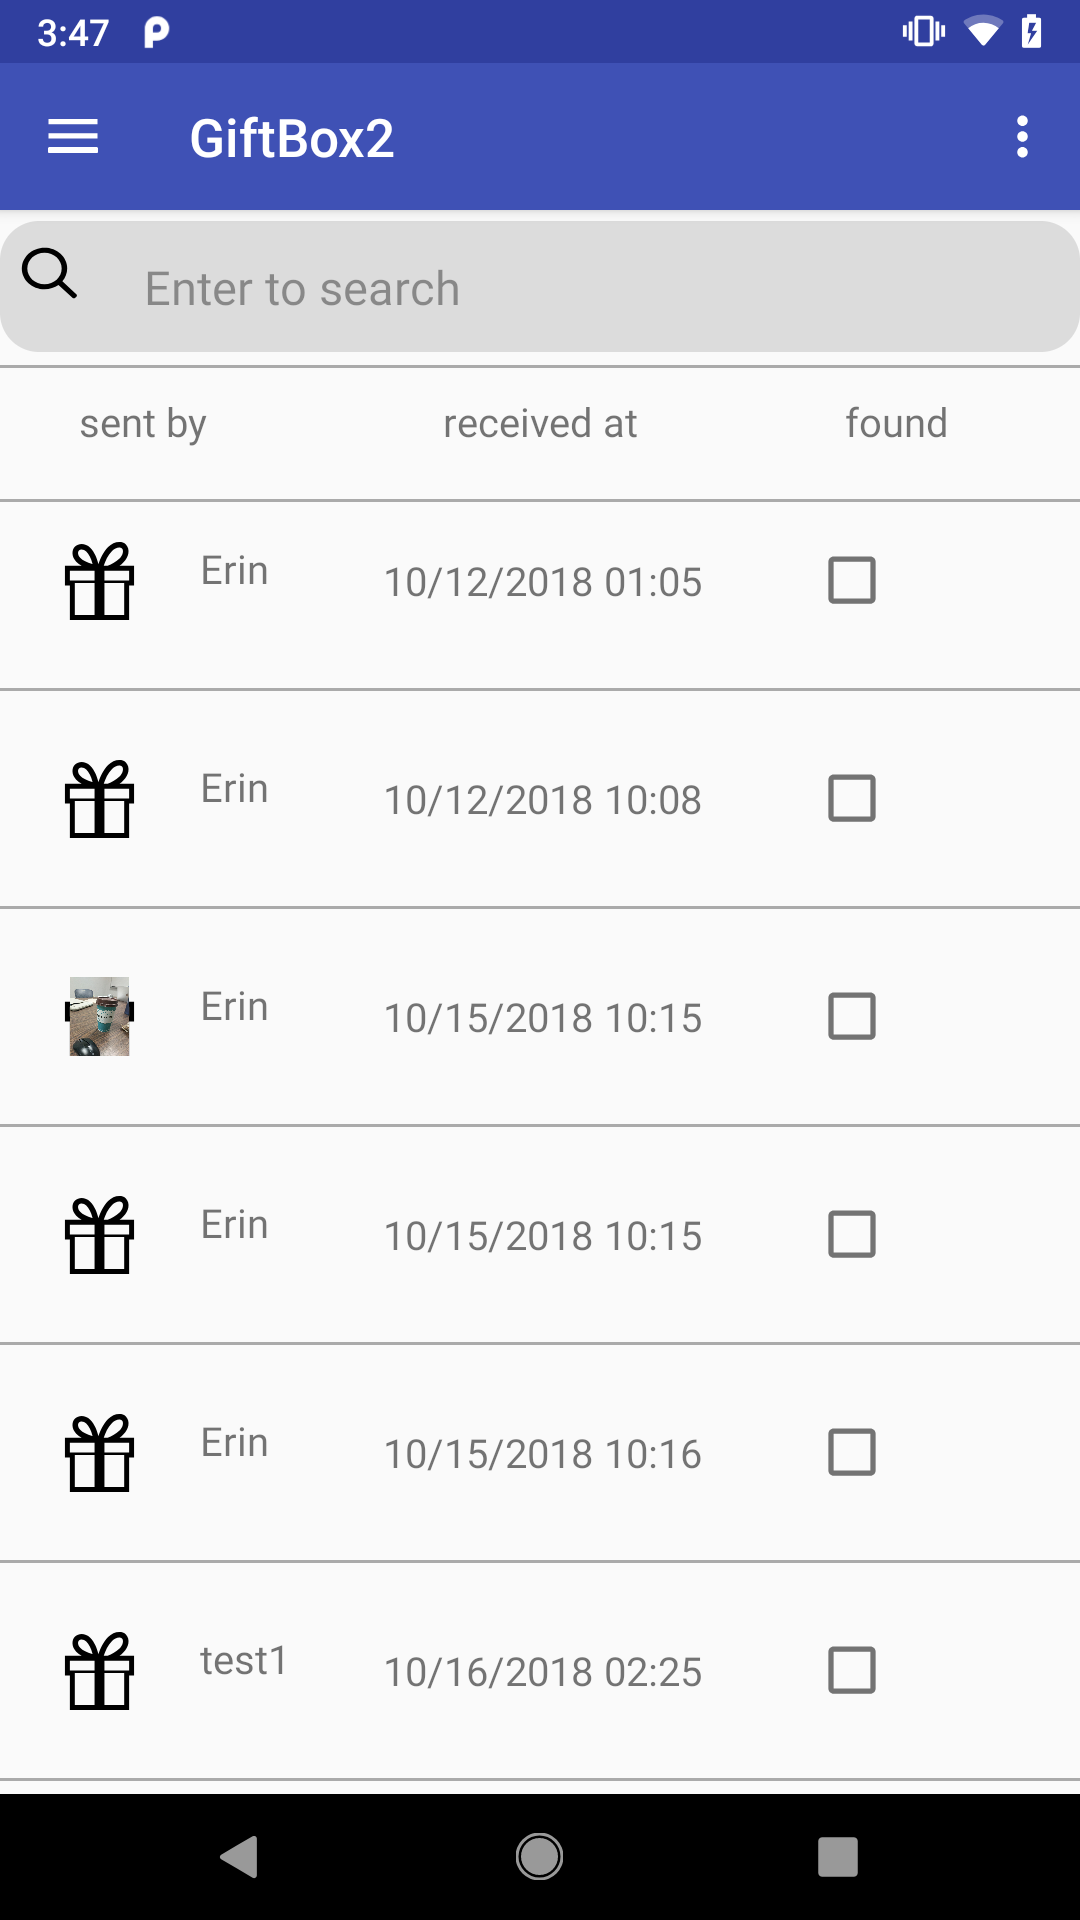
\includegraphics[width=.95\textwidth]{section03/assets/MainPage.png}
\subcaption{}
\end{minipage}%
\begin{minipage}[t]{0.5\textwidth}
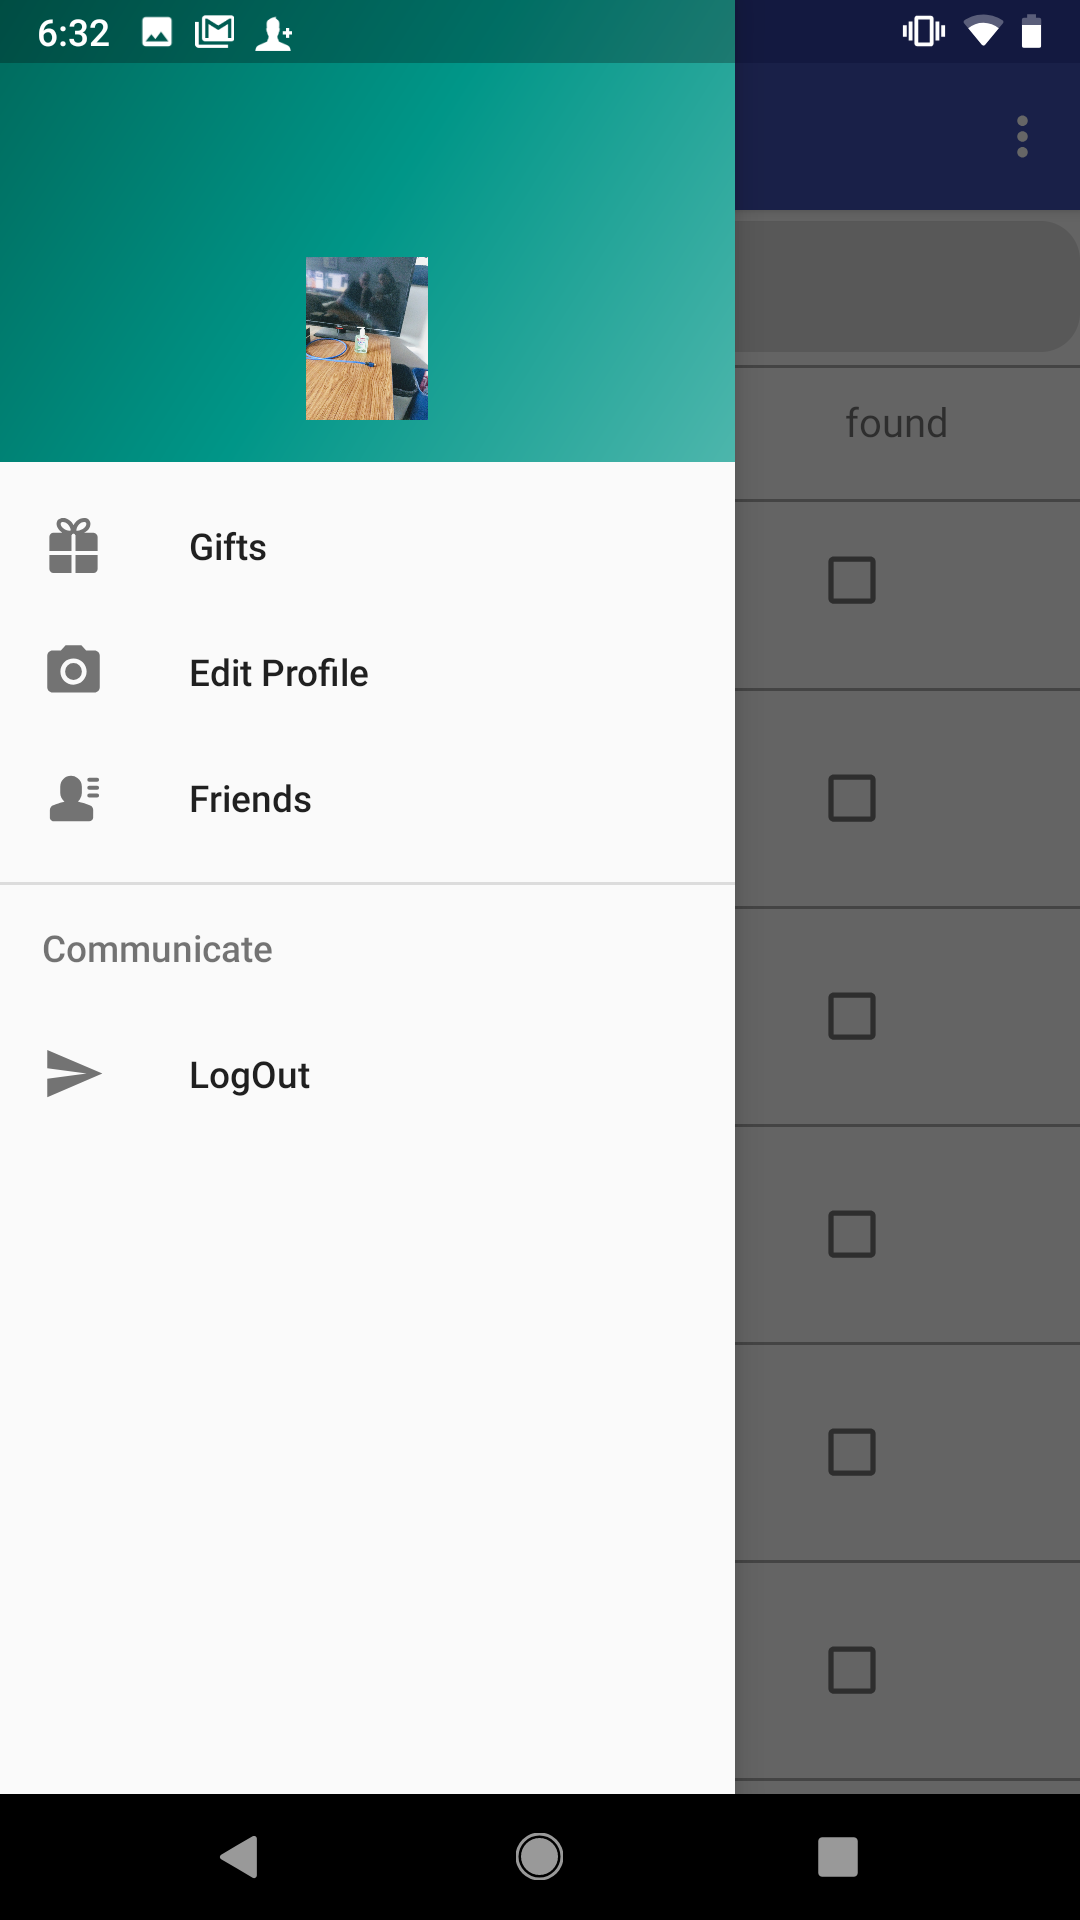
\includegraphics[width=.95\textwidth]{section03/assets/MainPortrait.png}
\subcaption{}
\end{minipage}%
\caption[Short Caption 2]{\label{MainPageUI}Main page}
\end{figure}

\begin{figure}[htb]
\centering
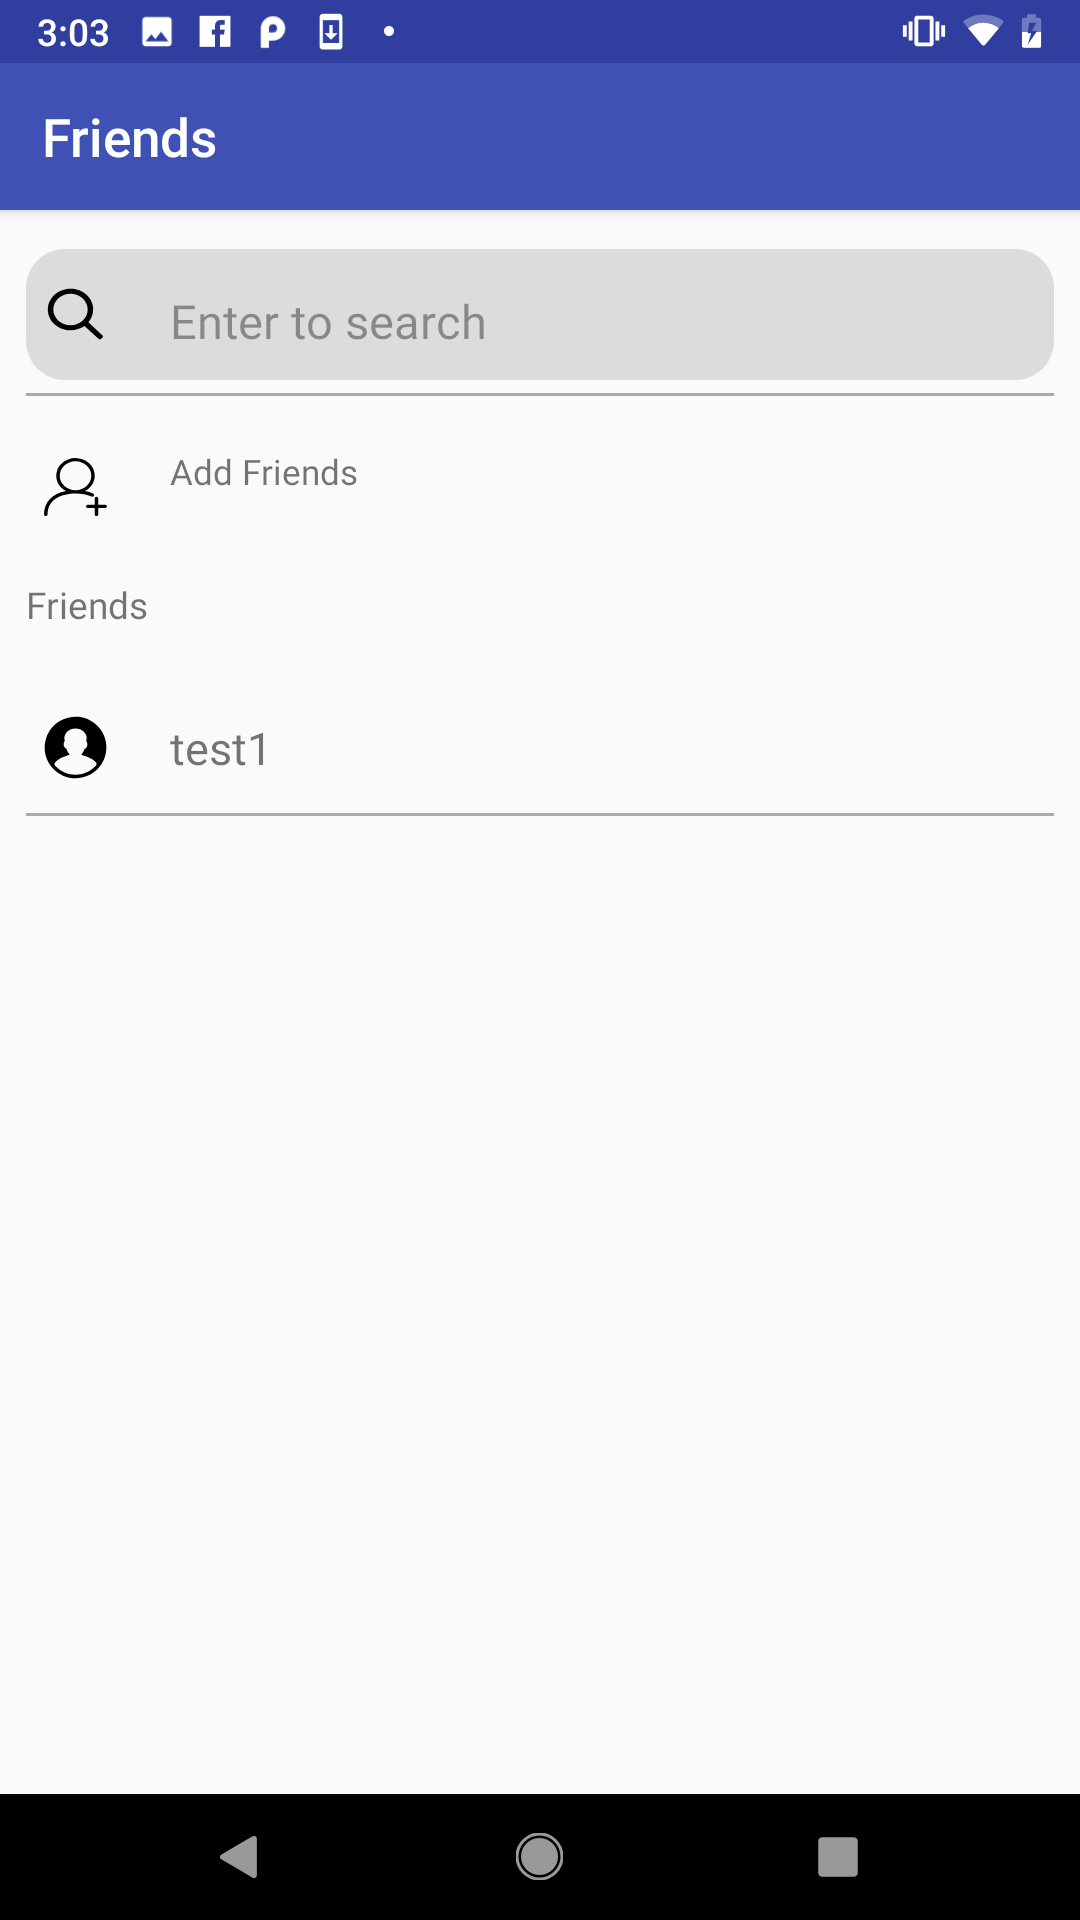
\includegraphics[width=.5\textwidth]{section03/assets/FriendsList.png}
\caption[Short Caption 2]{\label{FriendsListUI}Friends List page}
\end{figure}

\begin{figure}[htb]
\centering
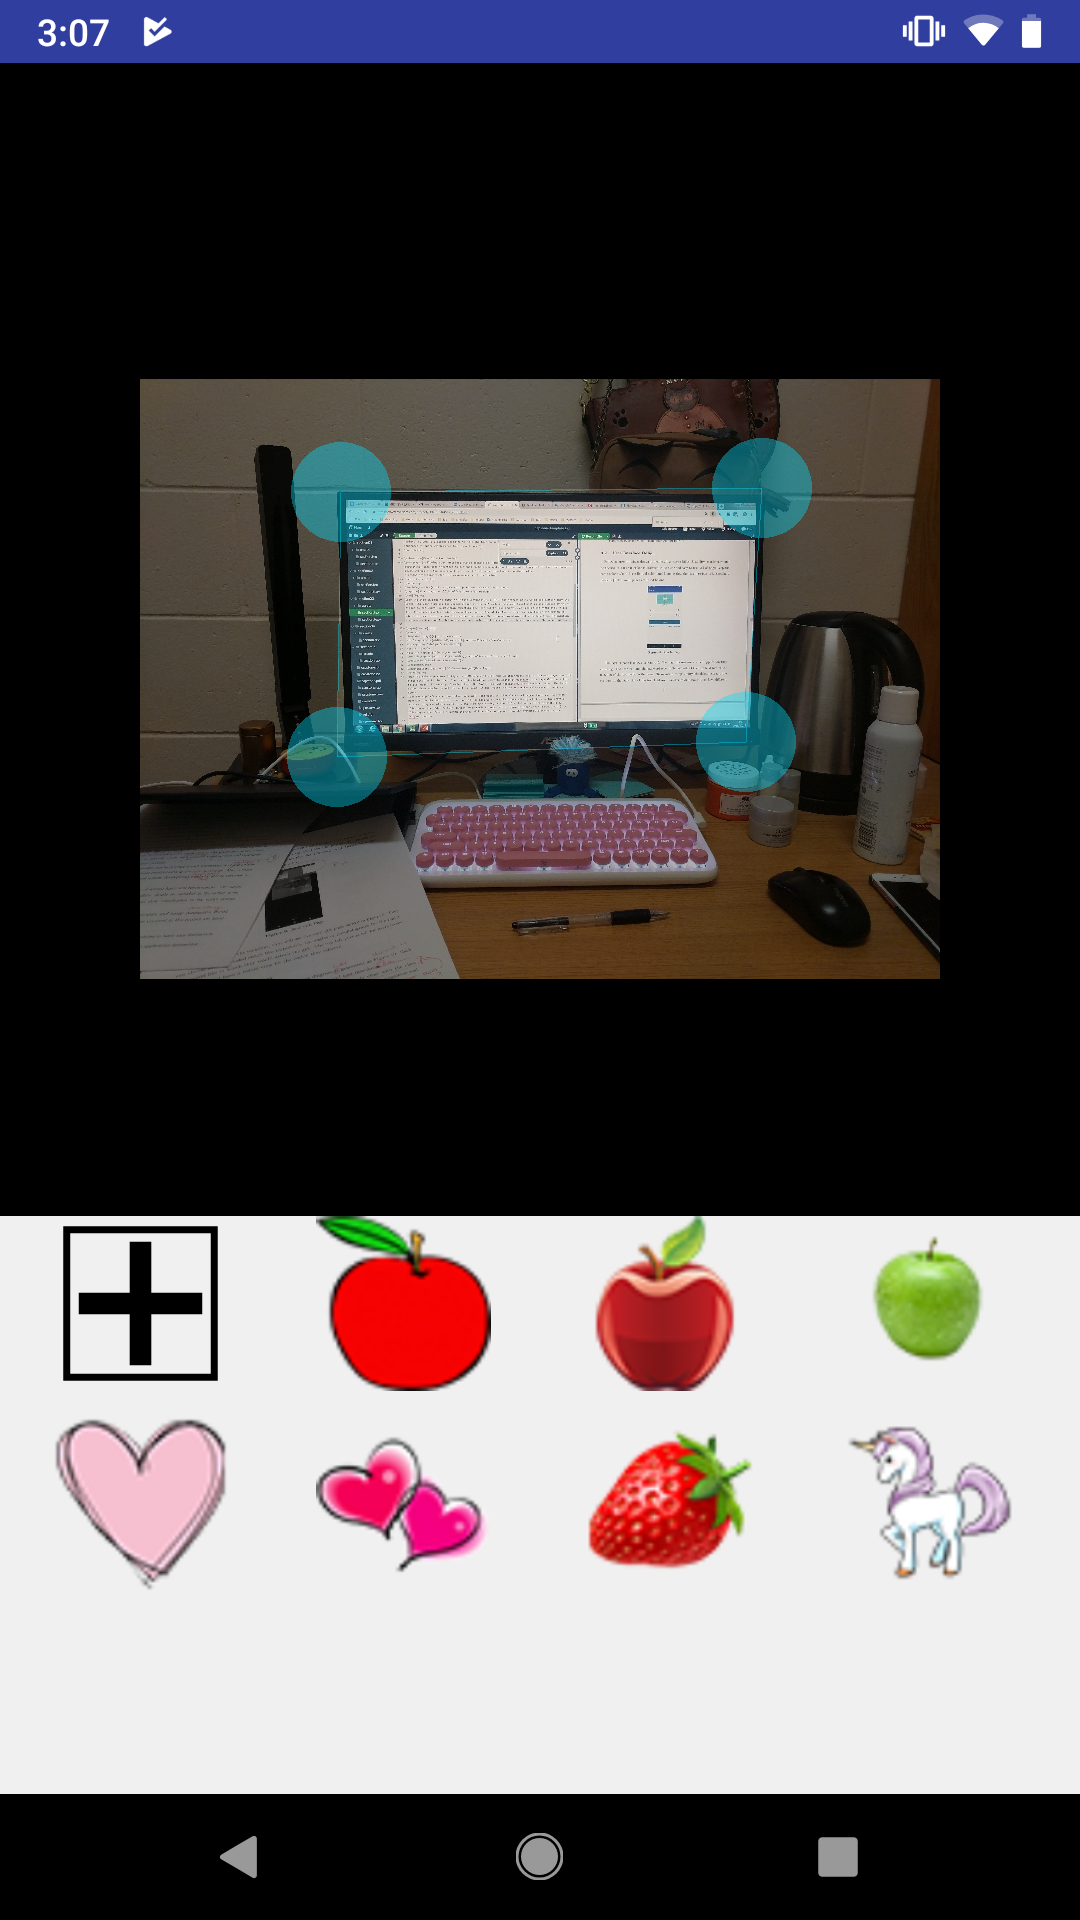
\includegraphics[width=.5\textwidth]{section03/assets/SendGift.png}
\caption[Short Caption 2]{\label{SendGiftUI}Send Gift Page}
\end{figure}

\subsection{Architecture Design}
There are 8 main classes designed for the whole project.
